% !TeX root = ../thuthesis-example.tex

\chapter{绪论}

\section{项目背景}

CPP2PY \cite{bestoftwo}是一个基于 Cython 的软件开发工具,用于简化为 C/C++ 程序编写 Python 接口的工作。本质上说,CPP2PY 是一个编译器,以 C/C++ 声明为输入,创建从 Python 语言调用这些声明所需的包装器。利用CPP2PY,使用者通常可以在几分钟内为小型 C/C++ 项目建立可用的 Python 接口,而不需要修改现有代码。该工程的可能应用包括:

\begin{itemize}
    \item 使用 Python 脚本或交互式命令行(IDLE 或 Jupyter notebook)测试 C/C++ 程序;
    \item 为 C/C++ 程序开发图形化的用户界面,如基于 Flask、Django 等 Python Web 框架;
    \item 为 Python 建立高性能的 C/C++ 模块;
    \item 快速原型设计。
\end{itemize}

为了说明本项目的潜力,有必要列举 C/C++ 编程的优势和痛点,让我们先从前者开始:

\begin{itemize}
    \item 性能优越;
    \item 系统级编程,比如在 C 语言中内嵌汇编指令;
    \item C++ 强大的抽象能力;
    \item 高度优化的编译器,分布广泛的用户社区和数不清的历史遗产。
\end{itemize}

总而言之,很多时候,C/C++ 都是不可替代的,这使得开发者不得不忍受 C/C++ 编程中的如下问题:

\begin{itemize}
    \item 编写用户界面并不容易;
    \item 软件测试的大量时间耗费在编译-调试循环中;
    \item 模块化机制复杂,缺乏通用包管理器,难以二次开发;
    \item 各种安全问题,如缓存区溢出等。
\end{itemize}

作为对比,在 Python 这样的脚本语言中,编写一个图形用户界面要容易得多;交互式的解释器也可能成为有用的调试和测试工具;数目庞大的第三方库可供选择,诸如 pip,conda 这样的包管理器让调用他人的代码简单又自然;开发者通常不必担心内存泄露问题,有自动垃圾回收器保驾护航……任何编程语言都不可能是完美的,但不同的编程语言提供了不同的优势。

当 Python 被用来控制 C/C++ 程序时,产生的系统往往如图 1 所示。在这种编程模型中,开发者使用 Python 语言驾驭较高的抽象层级,利用特定的脚本指令访问 C/C++ 程序的底层功能。这种双语言编程模式是非常强大的,因为它利用了每种语言的优势:C/C++ 能带来高效的性能,处理复杂的系统编程任务;Python 能提供快速原型设计、交互式调试和方便的高级数据结构。

通过将 Python 和 C/C++ 结合在一起,开发者可以充分利用二者的特点,大大简化软件开发的某些方面。将 C/C++ 整合到 Python 语言中,往往会带来更好的模块化设计、更少的代码、更大的灵活度、以及更高的生产力。

\begin{figure}
  \centering
  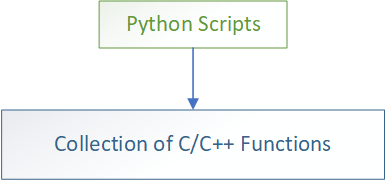
\includegraphics[width=0.5\linewidth]{figures/双语模型.png}
  \caption{Python - C/C++ 双语言编程模型}
  \label{fig:1}
\end{figure}

CPP2PY 最初是为了封装 C 稀疏矩阵算法库 SuiteSparse 中的稀疏分解算法而编写的。它以 libclang 为编译前端,Cython 为编译后端,解析 C/C++ 头文件生成 Cython 代码、构建文件和相应的 Python 存根文件。本项目在设计上避免生成过于复杂的代码,使用者可以方便地在生成结果的基础上进行二次开发。得益于 Cython,借助 CPP2PY 为 Python 编写 C/C++ 跨语言接口往往能享受高性能和良好的可扩展性。

\section{Python 的 C/C++ 扩展}

作为脚本语言,Python 的核心是 Python 解释器,也就是 CPython。解释器控制着 Python 脚本的执行和变量的访问。通过扩展解释器,可以添加新的命令和变量。CPython 提供了用于定义这种新命令的特殊接口,规定了这些新命令应该如何与解释器挂钩,这就是 CPython C API\cite{pyc}。

为了将新的 C/C++ 接口嵌入 CPython 中,需要编写一个特殊的包装函数,充当 Python 解释器与底层接口之间的粘合剂;然后向Python 解释器提供包装函数的名称、参数等信息。然而,直接以这种方式创建扩展模块费时费力,Python 官方文档建议, 尽可能使用第三方工具,如 Cython,SWIG,cffi 等,以更简单、更精致的方式为 Python 构建 C/C++ 扩展\footnote{“Third party tools like Cython, cffi, SWIG and Numba offer both simpler and more sophisticated approaches to creating C and C++ extensions for Python.”}。

\subsection{Cython}

作为本项目的起点,Cython 将在本文中多次出现。它包含两重含义,Cython 语言和 Cython 编译器。

Cython 语言\cite{O2015Cython, cython} 保留了 Python 的大部分语法,但额外支持调用 C 函数,支持为变量和类成员声明 C 类型。Cython 编译器将 Cython 代码编译为 C/C++ 代码,C/C++ 编译器再将这些代码编译为二进制形式的 Python 模块。以这种形式生成的扩展充分利用了静态类型信息,在性能上高度优化,与相应 C 程序相差无几。

除了高性能之外,Cython 的其它优势包括内置 Numpy C API、无运行时依赖等。作为编写高性能子模块的不二之选,Cython 被应用在 Python 数值计算、数据处理、机器学习等领域,著名第三方库如 scipy、pandas、sklearn 中都有它的身影。

作为一门小众语言,Cython 也存在一些缺陷,主要包括:

\begin{itemize}
    \item 缺少 IDE 支持,缺乏代码高亮、自动补全、自动格式化等开发工具;
    \item 作为一门语言来说,缺少系统完善的文档;
    \item 缺乏对 C++ 高级特性的支持。
\end{itemize}

CPP2PY 将 Cython 程序编写中的大部分任务自动化,能有效缓解其文档、辅助开发工具不足带来的不便。具体来说,利用 Cython 为 C/C++ 程序编写 Python 接口,通常需要三个步骤:

\begin{itemize}
    \item [1)] 罗列需要的 C/C++ 接口声明;
    \item [2)] 编写调用接口所需的 Cython 代码,根据需求进行扩展;
    \item [3)] 编写构建脚本,指定编译、链接参数。
\end{itemize}

这之中包含大量简单重复的工作,CPP2PY 正为此而生,它自动解析 C++ 头文件,生成接口声明和对应的包装代码,并自动生成构建脚本。

\subsection{与替代选择的比较}

除了 Cython 之外,还有其他第三方工具能为 C/C++ 程序编写 Python 接口,表 \ref{tab:1.2} 罗列了它们各自的特色\cite{msdnexperiment, cythonothers}。

\begin{table}
  \centering
  \caption{在 Python 中编写 C/C++ 扩展的可选方法}
  \begin{tabular}{lll}
    \toprule
     方法      &  创建年份  &  特色                           \\
    \midrule
     Cython    &  2007      &  高性能、NumPy 交互             \\
     PyBind11  &  2015      &  支持更多 C++ 高级特性          \\
     SWIG      &  1996      &  支持除 Python 外的其它目标语言 \\
     ctype     &  2003      &  Python 标准库                  \\
     cffi      &  2013      &  ctype 的替代选择,在运行时动态提供跨语言接口         \\
    \bottomrule
  \end{tabular}
  \label{tab:1.2}
\end{table}



其中,ctype 和 cffi 只支持 C 语言;PyBind11 和 SWIG\cite{swig} 要求开发者编写 C++ 代码指定封装的细节。而 Cython 与其它专为编写跨语言接口而生的竞争者不同,它是一门完整的编程语言,具有更强的可扩展性。

表 \ref{tab:1.3} 比较了支持 C++ 的各种第三方工具的性能。测试的方法是以各种工具包装用 C++ 编写的双曲正切函数 
\begin{equation}
    tanh(x) = \frac{e^x-e^{-x}}{e^x+e^{-x}}
\end{equation}
随机生成一千万个均匀分布于 $(-2,2)$ 之间的浮点数,通过跨语言接口计算其双曲正切函数值。由测试结果可知,Cython 在性能方面尤为突出,与直接使用 CPython C API 相差无几。

\begin{table}
  \centering
  \caption{不同扩展方式的性能比较}
  \begin{tabular}{ll}
    \toprule
     方法           &  用时 (s) \\
    \midrule
     纯 Python      &  4.939    \\
     CPython C API  &  1.210    \\
     Cython         &  1.254    \\
     PyBind11       &  2.464    \\
     SWIG           &  2.000    \\
    \bottomrule
  \end{tabular}
  \label{tab:1.3}
\end{table}

综合考虑各个工具的特点,可以得出以下结论:如果开发者对跨语言接口的性能有较高要求,或者希望利用 Numpy C API,应选择 Cython 作为开发工具;而如果希望尽可能保留 C++ 语言的高级特性,则可选用 PyBind11;如果需要在项目中使用第三种语言,则可选择 SWIG。值得一提的是,如果开发者只想加速 Python 代码,而不是封装已有的 C/C++ 程序,则应该先尝试 Numba,它为 Python 语言的一个子集和 NumPy 提供了 CPU 和 GPU 上的自动并行功能。

\section{相关工作}

Cython 百科\footnote{\url{https://github.com/cython/cython/wiki/AutoPxd}}列举了一些已有的且仍在维护中的同类型工具,包括 python-autopxd 和 autowrap,前者解析 C 头文件生成 Cython 声明,后者解析 Cython 声明生成包装代码。然而,本文的工作并未参考它们,从功能上说,本项目支持解析 C++ 语法,并能同时生成 Cython 声明和包装代码,与已有工具相比更加全面。

要将 C++ 程序迁移到 Python 中 会面临许多困难。首先,C++ 语法极为复杂,CPP2PY 依靠 libclang 来处理 C++ 头文件、分析类型系统;另外,C++ 与 Python 在很多方面有根本性的差异,许多 C++ 语法在 Python 或 Cython 中没有对应,CPP2PY 不得不采用一些折衷的方式处理它们。本文主要参考了 SWIG\cite{swig} (Simplified Wrapper and Interface Generator)对全局变量、类和重载的处理,详见第二章与第三章。CPP2PY 与 SWIG 的本质区别在于编译目标不同——CPP2PY 生成 Cython 代码,而SWIG 直接生成 C/C++ 代码。

\section{本文结构与贡献}

本文分为五个章节,第一章为绪论,介绍项目背景、技术路线和相关工作。

第二章介绍关键部分的设计、模块划分,以及软件测试情况。

第三章详细介绍了本程序的功能和使用方法。

第四章以稀疏矩阵库 SuiteSparse 中的稀疏矩阵 Cholesky 分解算法为例,介绍本项目的应用。

第五章为总结。

截至目前,CPP2PY 支持的特性包括:

\begin{itemize}
    \item 全局变量和宏;
    \item 基本数据类型及其指针、数组,部分 STL 容器;
    \item 枚举、联合、结构体与类;
    \item 类的静态成员、继承、运算符重载、抽象类;
    \item 默认参数、类型别名、异常、命名空间等;
    \item 生成对应 Python 存根文件,为二进制模块提供代码补全和类型注解。
\end{itemize}

所有这些特性及其限制将在第三章详细说明。本项目所有代码托管于 \url{https://github.com/zhanghx0905/cpp2py-cython}。 